\documentclass[a4paper, oneside]{book}
\usepackage{CJKutf8}
\usepackage{indentfirst}
\usepackage{graphicx}
\usepackage{multirow}
\usepackage{verbatim}
\usepackage[unicode=true]{hyperref}


\renewcommand{\tablename}{表}
\renewcommand{\figurename}{图}

\author{The Cytoscape Collaboration \\ Translated by Gang Chen}
\title{Cytoscape用户手册}
\date{\today}

\begin{document}
\begin{CJK}{UTF8}{msyh}
\maketitle
\tableofcontents

\chapter*{Cytoscape 2.6用户手册}
本文档遵守Creative Commons License,2006

作者:The Cytoscape Collaboration

中文翻译:Gang Chen <chengang@gossipcoder.com>

Cytoscape项目由以下单位合作:
\begin{itemize}
\item 加州大学圣地亚哥分校
\item 系统生物学研究中心
\item Memorial Sloan-Kettering癌症研究中心
\item Pasteur研究中心
\item 安捷伦科技公司
\item 加州大学旧金山分校
\end{itemize}

Cytoscape的资金来自NIH的美国国家通用医学研究中心(NIGMS),资金编号为:GM070743-01。整体资金通过来自Unilever PLC的合同提供。

\chapter*{引言}
Cytoscape~项目致力于为用户提供一个开源的网络显示和分析软件。软件的核心部分提供了网络显示、布局、查询等方面的基本功能。软件的核心可以通过插件架构进行扩展,这样就能快速地开发出新的功能。

Cytoscape源自系统生物学,用于将生物分子交互网络与高通量基因表
达数据和其他的分子状态信息整合在一起。虽然Cytoscape也能适用于
其他分子构件和相互作用,但其最强大的功能还是用于大规模蛋白质-
蛋白质相互作用、蛋白质-DNA和遗传交互作用的分析。各种物种,包括
人类,的这方面的实验数据都在迅速增加。通过Cytoscape,用户可以在可视化
的环境下将这些生物网络跟基因表达、基因型等各种分子状态信息整合
在一起,还能将这些网络跟功能注释数据库链接在一起。

Cytoscape~的核心是网络(图),其中的节点(~node~)是基因、蛋白质或分子,其中的连接则是这些生物结构之间的相互作用。

\section{开发}

Cytoscape~是~Institute for Systems Biology~(~Leroy Hood~实验室)、加州大学圣地亚哥分校(~Trey Ideker~实验室)、~Memorial Sloan-Kettering~癌症研究中心(~Chris Sander~实验室)、Pasteur研究院(Benno Schwikowski实验室)、安捷伦科技(Annette Adler实验室)和加州大学旧金山分校(Bruce Conklin实验室)的合作项目。

详情请访问http://www.cytoscape.org。

\section{授权}
Cytoscape~受~GNU LGPL~(~Lesser General Public License~)~的保护。在本手册的附录中能找到该授权,同时可以访问~http://www.gnu.org/copyleft/lesser.txt~。~Cytoscape~还是用了其他的一些开源程序库,详情见本手册的致谢。

\section{2.6版本的更新}
Cytoscape 2.6~中增加了很多新功能,在性能和软件的易用性上也有提升。包括:
\begin{itemize}
\item Web Service Client Manager框架能将Web服务客户端集成到Cytoscape中。
\item 通过Web服务客户端插件,可以从PathwayCommons、IntAct和NCBI Entrez Gene下载网络数据。
\item 通过Web服务插件,可以从BioMart导入注释信息。这主要是用于ID的翻译和名称映射。
\item Cytoscape主题。
Dynamic filters.
\item 动态过滤器。
Network Manager supports multiple network selection.
\item 网络管理器支持多网络选取。
Label Positioning has been improved.
\item 改进了标签的位置。
Session saving occurs in memory.
\item 将会话保存在内存中。
XGMML Improvements.
\item 改进了XGMML。
Network loading improvements.
\item 网络加载得到了改进。
\item Linkout integrated with attribute browser.
\item 通过可视化属性,引入了更多的Visual Style。
\item 修复了不计其数的bug。
\end{itemize}


\chapter{启动~Cytoscape}
Cytoscape~是一个Java程序,能在~Linux~、~Windows~和~Mac OS X~上运行。对于其他能安装Java 5的操作系统平台,比如以Solaris和FreeBSD为代表的UNIX,Cytoscape也能运行,但官方并对此提供支持。

\section{系统要求}
	Cytoscape~对系统的具体要求取决于所加载、查看和操作的网络的大小。

	\begin{table}[htbp]
	\label{tabel:2}
	\centering
	\begin{tabular}{|l|l|l|}
	\hline
	 & 小型网络查看 & 大型网络分析和查看 \\
	\hline
	处理器 & 1GHz & 尽可能的快\\
	\hline
	内存   & 512MB & 2GB以上 \\
	\hline
	显卡   & 板载集成显卡 & 高端独立显卡 \\
	\hline
	显示器 & XGA($1024 \times 768$) & 高分辨率或双显示器 \\
	\hline
	\end{tabular}
	\caption{}
	\end{table}

\section{入门}
	\subsection{安装~Java}
		如果计算机上还没有安装~Java,那么首先要下载并安装~Java SE 5~或~6~。\textbf{Cytoscape~从2.5版开始就不能在~Java 1.4~上运行。必须安装~Java SE 5~或~6~!!!}
		Java SE 5~和~Java SE 6可以从这里下载:
		\begin{itemize}
		\item \href{http://java.sun.com/javase/downloads/index_jdk5.jsp}{Java SE 5}
		\item \href{http://java.sun.com/javase/downloads/index.jsp}{Java SE 6}
		\end{itemize}
	
		一般情况下,Java SE 6~的运行速度要快一些。所以,如果您的计算机兼容~Java SE 6~的话,请尽量使用~Java SE 6。

	\subsection{安装~Cytoscape}
		Cytoscape~供下载的版本很多,安装方法也不尽相同。所有的版本都可以从~http://cytoscape.org~网站下载。
		
		\begin{itemize}
		\item Windows、Mac OS以及Linux平台上的自动安装包
		\item 压缩发行版
		\item 从源代码编译
		\item 从Subversion源中提取最新版的软件
		\end{itemize}

		Cytoscape的安装目录(无论是什么平台)中包含表~\ref{table:3}~中的文件。

		\begin{table}[!h]
		\begin{tabular}{|l|l|}
			\hline
			文件 & 描述 \\
			\hline
			cytoscape.jar & Cytoscape~的主程序(~Java~压缩包)。\\
			\hline
			\multirow{2}{*}{cytoscape.sh} & 从命令行运行~Cytoscape~的脚本(用于~Linux~和~\\&Mac OS X~)。\\
			\hline
			cytoscape.bat & 运行Cytoscape的脚本(用于~Windows~)。\\
			\hline
			LICENSE.txt/html & Cytoscape GNU LGPL~授权。\\
			\hline
			lib/ & Cytoscape运行所需的jar库。\\
			\hline
			docs/ & 各种格式的用户手册。也就是你正在阅读的东西。\\
			\hline
			plugins/ & jar格式的Cytoscape插件。\\
			\hline
			sampleData/ & \\
			\hline
				& galFiltered.gml -- 分子相互作用网络数据示例$^*$。\\
			\hline
				& galFiltered.sif -- Simple Interaction~格式的同一个网络$^*$\\
			\hline
				& galExpData.pvals -- 基因表达矩阵文件示例$^*$。\\
			\hline
				\multirow{2}{*}{} & galFilteredAttrTable.xls -- 微软~Excel~格式的节点属性\\ & 文件示例。\\
			\hline
				\multirow{2}{*}{} & galFiltered.sif -- 用上面的数据库和多个注释数据库创建\\ & 的会话示例$^*$。\\
			\hline
				\multirow{2}{*}{} & BINDyeast.sif -- BIND数据库中酵母的蛋白质相互作用\\ & 网络,2006年12月$^{**}$。\\
			\hline
				\multirow{2}{*}{} & BINDhuman.sif -- BIND数据库中人类的蛋白质相互作\\ & 用网络,2006年12月$^{**}$。\\
			\hline
				& yeastHighQuality -- 分子生物相互作用的示例文件$^{***}$。\\
			\hline
				\multirow{2}{*}{} & interactome\_{}merged\_{}networkTable.gz -- 制表符分割格\\ & 式的人类相互作用网络$^{****}$。\\
			\hline
				& sampleStyle.props -- 附加的~Visual Sytle~示例。\\
			\hline
		\end{tabular}
		\caption{$^*$ 来自~Ideker er al, Science 292:929 (2001); $^{**}$ 来自~http://www.blueprint.org/bind/bind\_{}downloads.html; $^{***}$ 来自~Mering et al, Nature, 417:399 (2002) Lee et al, Science 298:799 (2002);$^{****}$来自~Cytoscape~教程网页。原始数据可以从~http://cytoscape.org/cgi-bin/moin.cgi/Data\_{}Sets/上由Andrew Garrow、Yeyejide Adeleye和Guy Warner(Unilever, Safety and Enviromental Assurance Center)创建的“A merged human interactome”中下载。 }
		\label{table:3}
		\end{table}

	\subsection{启动程序}
		双击安装程序创建的图标,或是在命令行中运行~cytoscape.sh(Linux或Mac OS X),也可以双击~cytoscape.bat(Windows)~就能启动~Cytoscape。还可以在命令行中将这个jar文件以命令行参数的形式传递给命令~java -Xmx512M -jar cytoscape.jar -p plugins~。~-Xmx512M~标志是告诉~java~给~Cytoscape~分配较多的内存,~-p plugins~则是告诉~Cytoscape~加载~plugins~目录中所有的插件。插件对于~Cytoscape~是非常重要的,诸如布局(layout)、过滤器(filter)和属性浏览器之类的功能都是由插件提供的。关于命令行参数的详细信息请阅读\textit{命令行参数}一章。在~Windows~中,只需要双击~jar~文件就能启动~Cytoscape。不过,这样就不能使用命令行参数了(比如制定插件目录的位置)。

		成功地启动~Cytoscape后,就会看到如图~\ref{fig:1.1}~所示的窗口(图~\ref{fig:1.1}~来自Mac OS 10.4)。

		\begin{figure}[h]
			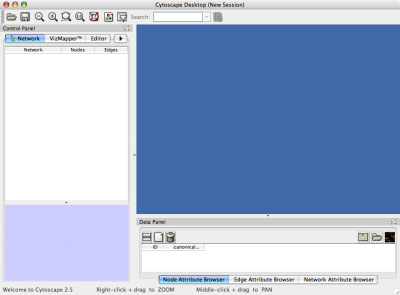
\includegraphics[width=\textwidth]{images/cytoscape_startup_mac.png}
			\caption{Cytoscape启动界面}
			\label{fig:1.1}
		\end{figure}

		\subsubsection{注意内存使用量}

		随着用用户所加载的网络的规模的增加,Cytoscape所需的内存也会增加。内存的使用量取决于网络对象(节点和边)的数量以及属性的数量。表~\ref{table:4}~和~\ref{table:5}是对内存需求量的粗略估计。

		\begin{table}[htbp]
		\centering
		\begin{tabular}{|l|l|}
			\hline
			对象的数量(节点和边) & 建议内存\\
			\hline
			0 -- 70,000 & 512M(默认值)\\
			\hline
			70,000 -- 150,000 & 800M \\
			\hline
		\end{tabular}
		\caption{无视图情况下的建议内存大小}
		\label{table:4}
		\end{table}

		\begin{table}[htbp]
		\centering
		\begin{tabular}{|l|l|}
			\hline
			对象的数量(节点和边) & 建议内存\\
			\hline
			0 -- 20,000 & 512M(默认值)\\
			\hline
			20,000 -- 70,000 & 800M \\
			\hline
			70,000 -- 150,000 & 1G \\
			\hline
		\end{tabular}
		\caption{有视图情况下的建议内存大小}
		\label{table:5}
		\end{table}

		\subsubsection{Cytoscape的整体内存需求}
		可以通过命令行参数增加Cytoscape的内存大小。例如,如果要给Cytoscape分配1G的内存,可以在命令行输入:
		\begin{verbatim}
		java -Xmx1GB -jar cytoscape.jar -p plugins
		\end{verbatim}

		\subsubsection{堆栈尺寸(stact size)}
		这是另一个跟内存分配有关的选项。Cytoscape的部分功能需要较大的堆栈空间(某些操作所需的临时内存,比如Layout)。由于这个堆栈的大小是独立于前面的Xmx值的,所以有时候Layout算法会因为内存不足而失败。为了避免这种情况,可以用-Xss制定更大的堆。如果对大型网络布局时失败,可以尝试下面的命令:
		\begin{verbatim}
		java -Xmx1GB -Xss10M -jar cytoscape.jar -p plugins
		\end{verbatim}
		选项-Xss10M的意思就是将堆的尺寸设置为10MB。在大部分情况下,这能解决由于内存不足导致的Layout问题。

		\begin{figure}[!h]
		\centering
		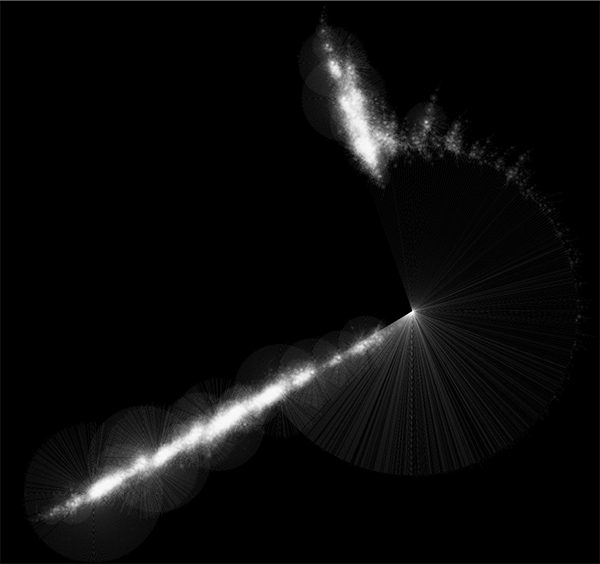
\includegraphics[width=\textwidth]{images/one_million_network.png}
		\end{figure}


\chapter{Cytoscape快速入门}
加载了网络之后,~Cytoscape~的界面如图~\ref{fig:2.1}~所示。

\begin{figure}[!h]
\centering
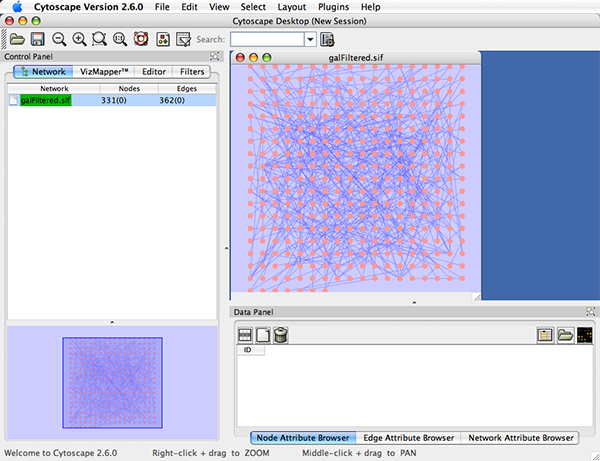
\includegraphics[width=\textwidth]{images/cytoscape_startup_network_26.png}
\caption{~Cytoscape~加载网络后的界面截图}
\label{fig:2.1}
\end{figure}

主界面由多个组件构成,包括:
\begin{itemize}
\item 顶部的菜单(稍后会对各个菜单做详细介绍)。
\item 工具栏,包含了各种常用功能。从菜单中也能使用这些功能。鼠标指针在这些图标上停留片刻就能看到有关的提示。
\item 网络管理面板(左上方的面板)。其中有可关闭的网络全局浏览面板(左下方)。
\item 网络查看主窗口,网络就显示在这个窗口中。
\item 属性浏览器面板(底部的面板),显示所选择的节点和边的属性。在这个面板中还可以对这些属性的值进行修改。
\end{itemize}

网络管理和属性浏览器面板是可以拖拽的标签面板,被称为~CytoPanels~。通过点击~CytoPanel~右上角的浮动窗口(Float Window)控件~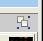
\includegraphics{images/float_icon.png}~可以将这些面板设为浮动状态。

如果选择了这个控件,例如属性浏览器面板上的这个控件,就会出现两个~Cytoscape~的窗口,一个是主窗口,另一个是名为CytoPanel 2的新窗口,如下图所示。当鼠标指针指向单元格时,会看到弹出信息。

{\centering
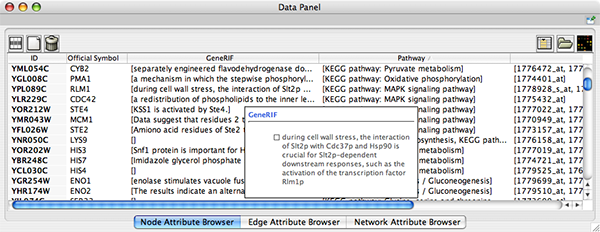
\includegraphics[width=\textwidth]{images/attribute_browser_26.png}
}

在图中可以看到,CytoPanel 2~现在有一个~Dock Window~控件。如果点选这个控件,这个窗口就会回到主窗口中。

Cytoscape~还提供了一个用于构建和编辑网络的编辑器,把面板中的节点和边拖拽到主网络视图窗口中就能创建和编辑网络。用Visual Style可以定义节点的形状以及边的箭头。只需要选择CytoPanel 1中的Editor标签就能编辑网络。下图展示了一个编辑器,Visual Style是BioMoleculeEditor。

{\centering
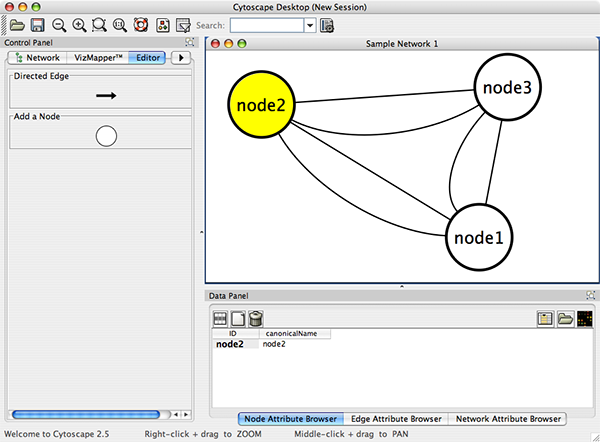
\includegraphics[width=\textwidth]{images/editor_25.png}}

\section{菜单}
	\subsection{File}
	File菜单中含有最基本的文件操作功能:File $\rightarrow$ Open~用于打开~Cytoscape~会话文件;File $\rightarrow$ New~用于新建空白网络,也可以从现用的网络创建新网络;File $\rightarrow$ Save~用于保存会话文件;File $\rightarrow$ Import~用于导入网络或属性数据;File $\rightarrow$ Export~用于导出数据和图片。File $\rightarrow$ Print用于打印,File $\rightarrow$ Quit~则是关闭所有的~Cytoscape~窗口,并推出程序。

	\begin{figure}[!h]
	\centerline{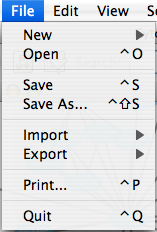
\includegraphics[scale=0.6]{images/menu_file_26.png} }
	\end{figure}

	\subsection{Edit}
	Edit菜单中提供了用于属性浏览器、网络编辑器和布局的撤销(Undo)和重做(Redo)功能。
	
	还有创建和销毁视图(网络的显示方法)和网络(网络的原始数据,并不可视化的)的菜单项,以及用于从当前网络中删除所选节点和边的菜单项。通过 Edit $\rightarrow$ Undo~可以恢复被删除的节点和边。配置和插件的设置可以通过Edit $\rightarrow$ Preferences $\rightarrow$ Properties来编辑。

	\begin{figure}[!h]
	\centerline{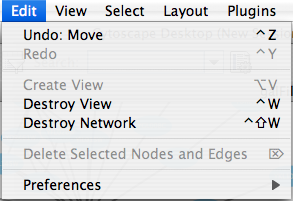
\includegraphics[scale=0.6]{images/menu_edit_26.png}}
	\end{figure}

	\subsection{View}
在~View~菜单中可以控制网络管理面板(CytoPanel 1)、属性浏览器(CytoPanel 2)、网络概览(在CytoPanel
1中)和VizMapper的显示和隐藏。

	\begin{figure}[!h]
	\centerline{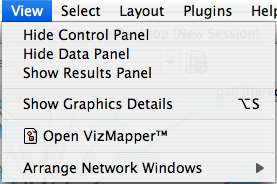
\includegraphics[scale=0.6]{images/menu_view_26.png}}
	\end{figure}

	\subsection{Select}
	在~Select~菜单中含有选择节点和边的各种选项。还有Select $\rightarrow$ Use Filter选项,用于根据节点或边的某些属性创建自动的过滤器。

	\begin{figure}[!h]
	\centerline{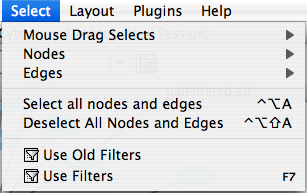
\includegraphics[scale=0.6]{images/menu_select_26.png}}
	\end{figure}

	\subsection{Layout}
	通过~Layout~菜单可以控制网络显示的形式。该菜单上半部分(Rotate,Scale,Align and
	 Distribute)是用于控制网络的显示。菜单的下半部分是用于自动布局网络的各种布局算法。

	\begin{figure}[!h]
	\centerline{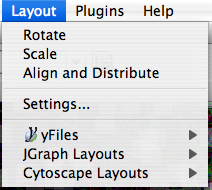
\includegraphics[scale=0.6]{images/menu_layout_25.png}}
	\end{figure}
	
		
	
	\subsection{Plugins}
	Plugins~菜单中提供了插件管理功能(安装、升级和删除),以及插件所添加的选项,比如
	~Agilent Literature Search~或~Merge Networks~。具体的内容取决于所加载的插件。
	\footnote{注意:在~\href{http://cytoscape.org/plugins2.php}
	{http://cytoscape.org/plugins2.php}~上有Cytoscape~插件的介绍。}
	
	\begin{figure}[!h]
	\centerline{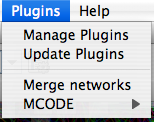
\includegraphics[scale=0.6]{images/menu_plugins_25.png}}
	\end{figure}
	
	\subsection{Help}
	在Help菜单中可以打开在线帮助,浏览本手册内容。“About...”则会显示正在运行的~Cytos
	cape~的版本信息。
	\begin{figure}[!h]
	\centerline{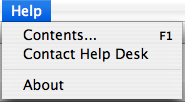
\includegraphics[scale=0.6]{images/menu_help_25.png}}
	\end{figure}

\section{网络管理}
	Cytoscape~2.3之后的版本都可以同时加载多个网络,有无视图都可以。网络中存放着用户
	加载所有节点和边,以及用户做指定的视图。同一个网络可以有多个视图。网络(以及相应
	的视图)可以有序地组织在一起。

    下图中展示了多个网络同时加载,并按层次结构组织的例子:

    \begin{figure}[!h]
    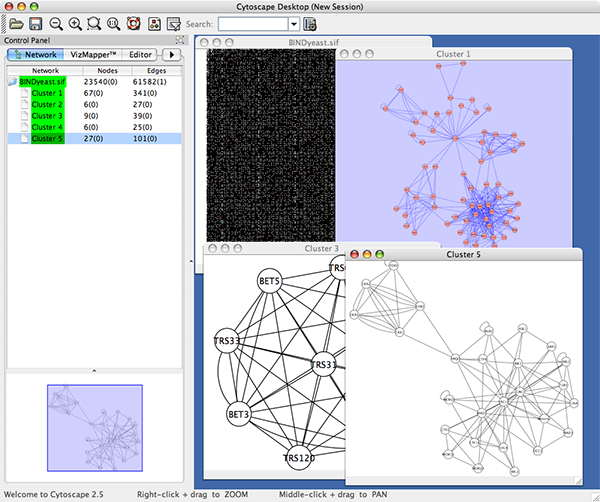
\includegraphics[width=\textwidth]{images/cytoscape_network_hierarchy_25.png}
    \end{figure}

    网络管理器(CytoPanel 1右上方的树状显示窗口)展示了当前所加载的网络。点击其中的
    网络就会在主窗口里面显示该网络的视图。在网络管理器中会显示各个网络的名称和尺寸(
    节点和边的数量)。如果网络是从文件中加载的,网络的名称就是文件名。
    
    对于那些规模较大的网络(数千个点和边),需要较长的时间才能显示出来。正因为如此, 
    Cytoscape中的网络可以不包含“视图”(View)。带有视图的网络以绿色高亮显示,而没有
    视图的网络则以红色高亮显示。在网络管理器中网络的名称上点击鼠标右键,就能创建或是
    销毁视图,通过Edit菜单也能实现同样的操作。用同样的方法可以销毁已加载的网络。在上
    图中,加载了七个网络,其中六个绿色的是有视图的,而红色的那个则是没有视图的 
    。\footnote{译者注:图中总共只有六个网络,都是绿色的,似乎原文有误。}

Cytoscape中的某些特定操作会创建出新的网络。如果新网络是从原有的网络中创建的,例如选择
原网络中的部分节点,将这些节点复制到新网络中(用File~$\to$~New~$\to$~Network option),
在这种情况下新网络就会显示为原网络的子网络。Cytoscape的这种显示方法使得用户能很快地
看出网络间的关系。上图中树顶部的那些网络就是这样生成的。

The available network views are also arranged as multiple overlapping windows in
the network view window. You can maximize, minimize, and destroy network views by
using the normal window controls for your operating system.

    \subsection{网络窗口排列}


\section{网络概览窗口}
	






\chapter{命令行参数}
Cytoscape~可以接受很多命令行参数,包括指定网络文件、属性文件和会话文件。下面的内容是用
Cytoscape~的“-h”或“--help”运行参数得到的:
\begin{verbatim}
usage: java -Xmx512M -jar cytoscape.jar [OPTIONS]
 -h,--help               Print this message.
 -v,--version            Print the version number.
 -s,--session <file>     Load a cytoscape session (.cys) file.
 -N,--network <file>     Load a network file (any format).
 -e,--edge-attrs <file>  Load an edge attributes file (edge attribute format).
 -n,--node-attrs <file>  Load a node attributes file (node attribute format).
 -m,--matrix <file>      Load a node attribute matrix file (table).
 -p,--plugin <file>      Load a plugin jar file, directory of jar files,
                         plugin class name, or plugin jar URL.
 -P,--props <file>       Load cytoscape properties file (Java properties
                         format) or individual property: -P name=value.
 -V,--vizmap <file>      Load vizmap properties file (Java properties format).
\end{verbatim}

在指定文件时,可以是本地文件的路径,也可以是URL。例如,可以这样指定本地的网络文件(假
设myNet.sif位于当前工作目录):cytoscape.sh -N myNet.sif。还可以用URL指定网络:
cytoscape.sh -N http://example.com/myNet.sif。
\begin{description}
\item[参数] 用途
\item[-h,--help] 显示上面已经展示过的帮助信息,然后退出程序。
\item[-v,--version] 显示~Cytoscape~的版本号,然后退出程序。

\item[-s,--session $<$file$>$] 这个选项用于加载指定的会话文件。
由于会话文件只能在特定的时间加载,所以这个选项在命令行中只能使用一次。要给这个选项指
定一个.cys~的~Cytoscape~会话文件。不过,cys~后缀并不是必须的。
\item[-N,--network $<$file$>$]
这个选项用来加载各种类型的网络文件,包括~SIG~、~GML~和~XGMML的各种格式的文件都可以通过- N
选项加载到~Cytoscape~中。在一个命令中可以同时加载多个网络。
\item[-e,--edge-attrs $<$file$>$] 这个选项用来指定边属性文件。
在一个命令中可以同指定多个边属性文件。
\item[-n,--node-attrs $<$file$>$] 这个选项用于指定节点属性文件。在一个命令中可以同指定多个边属性文件。
\item[-m,--matrix $<$file$>$]这个选项用于指定数据矩阵文件。
如果是用于生物网络分析,这个数据矩阵的内容就是基因表达数据。所有的数据矩阵文件都会以
节点属性的形式读入Cytoscape。在一个命令中可以同指定多个数据矩阵文件。
\item[-p,--plugin $<$file$>$]这个选项用于将指定的Cytoscape插件(.jar)文件加载到
Cytoscape中。老版本中的“资源插件选项(resource plugin option)”已经合并到了这个选项
中\footnote{这句话的翻译不确定,请有了解老版本Cytoscape的同学指正}。如果插件位于
Cytoscape的CLASSPATH路径中,还可以用类名称来制定插件。例如,假设能在~CLASSPATH~中找
到名为~MyPlugin~的类,那么就可以这样指定插件:cytoscape.sh -p MyPlugin.class。最后
一种指定插件的方面就是指定一个文本文件,在这个文本文件中列出所有需要加载的插件的~jar~文件名。 
\item[-P,--props
$<$file$>$]这个选项可以用来指定~Cytoscape~的各项属性。可以用过属性文件(格式是标准的
~Java~属性格式),也可以用等号设置单个属性的值。例如,指定缺省的物种:
cytoscape.sh -P defaultSpeciesName=Human。如果属性中有空格,加上引号就可以了,例如:
cytoscape.sh -P "defaultSpeciesName=Homo Sapiens"。
这个选项可以用来代替以前的-noCanonicalization,-species和-bioDataServer选项。现在的
命令可以写成这样的:cytoscape.sh -P defaultSpeciesName=Human -P noCanonicalization=true
-P bioDataServer=myServer.
\item[-V,--vizmap $<$file$>$] 这个选项用来指定可视化属性文件。
\end{description}

上面介绍的这些属性(包括插件)都可以在正在运行的Cytoscape的GUI中加载。

\chapter{Cytoscape~设置}
\section{管理属性}
\footnote{{\bf 重要:}如果你用过老版本的~Cytoscape就会发现属性的处理方式已经发生了
改编。其中,最重要的变化是属性不再是存放在当前目录或主目录的.cytoscape目录中,而是
保存在Cytoscape的会话文件中(后缀是.cys)。在.cytoscape目录下肯定会有一个
cytoscape.props文件,但这个文件只有当用户要求将但前属性保存为缺省属性时才会被修改。
除非实在是有什么特别的原因,否则还是用缺省设置比较好。}

用菜单上的Edit → Preferences → Properties…可以打开Cytoscape的属性编辑器,在这里可以
修改各种属性。对于一般的属性,都是保存在Cytoscape的会话文件中,所以只对当前会话有效。
只有将其设为缺省属性,或是用File → Export将其导出,才能在其他的会话中生效。

可以通过Add(添加)、Modify(修改)和Delete(删除)操作来配置Cytoscape的属性。
\begin{center}
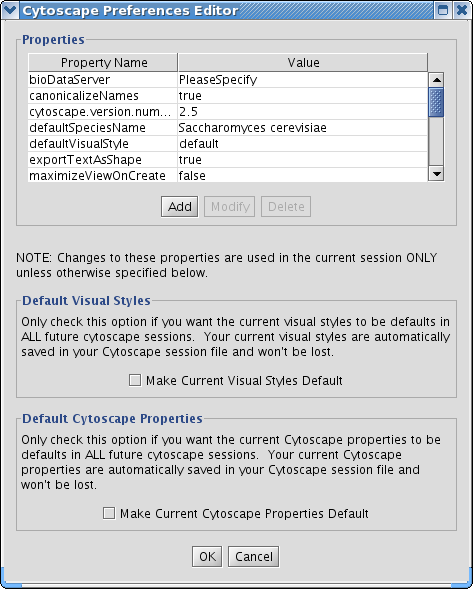
\includegraphics[width=\textwidth]{images/prefs_editor.png} 
 \end{center}

\chapter{创建网络}
在Cytoscape中有四种创建网络的方法:
\begin{enumerate}
\item 导入预设的格式化网络文件。
\item 导入预设的未格式化的文本文件或Excel文件。
\item 从Web Service导入网络。
\item 创建一个空网络,然后手动地添加节点和边。
\end{enumerate}
\section{导入确定格式的网络文件}

在\ref{ch06}中介绍的所有网络文件格式都可以导入到Cytoscape中。点击File $\rightarrow$ Import $\rightarrow$ Network (multiple file types),在弹出的``Import Network''窗口中就可以把网络文件导入到Cytoscape中。可以是本地计算机上的网络文件,也可以是远程计算机上的(用URL)。

 \subsection{从本地计算机上导入网络}
在缺省情况下,Cytoscape会从本地计算机加载网络。

在Import Networks中会显示缺省的``Data Source Type: Local,'',意思就是从本地计算机导入网络文件。 点击Select按钮选择要加载的网络文件(只有Cytoscape能识别的文件才会显示出来),然后点击Import按钮把网络加载到Cytoscape中。在Cytoscape的sampleData的文件夹中能找到一些不同类型的网络文件。 

SIF、GML和XGMML格式的网络文件也可以在命令行中用-N选项直接导入。

\begin{center}
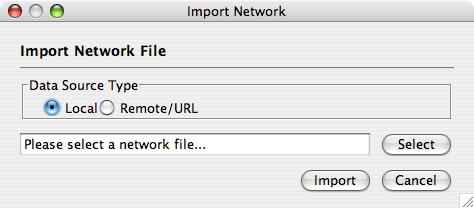
\includegraphics[width=.6\textwidth]{images/network_import_dialog1_25.png} 
\end{center}

\subsection{从远程计算机上导入网络(URL导入)}
在Import Networks中还可以使用URL导入网络文件。首先把Data Source Type设置成Remote,然后手动填写或是用书签插入合适的URL。点击文本域右边的箭头就能访问收藏的URL。(书签管理器的详细信息参阅Preferences中的Bookmark Manager一节。还可以把浏览器中的URL拖拽到URL文本框中。指定好URL后,点击Import按钮就能加载网络。

\begin{center}
 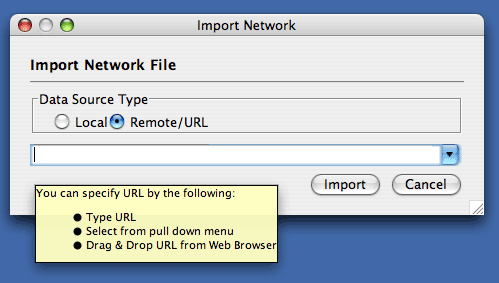
\includegraphics[width=.6\textwidth]{images/network_import_dialog2_25.png} 
\end{center}

从URL地址导入网络一定要注意一点。由于Cytoscape主要(但不是完全)是根据文件的后缀来判断文件的类型,所以如果URL中的文件的后缀不合适的话,在导入网络时就有可能遇到麻烦。如果Cytoscape没能在URL识别出有意义的文件名和后缀,它就会根据MIME类型来猜测文件的类型。如果所有的导入句柄就无法识别MIME类型,导入就会失败。

在导入网络时有可能遇到的另一个问题就是防火墙,导致无法访问文件。为了解决这个问题,Cytoscape支持使用代理服务器。在 Edit $\rightarrow$ Preferences$\rightarrow$ Proxy Server...中就可以设置代理服务器。在Preference有这方面的更多信息。

\section{导入格式灵活的表格文件}
\label{free-format table}
从2.4版开始,Cytoscape就能通过Edit $\rightarrow$ Import $\rightarrow$ Network from Table (Text/MS Excel)...从文本文件和Excel文件中导入网络。在弹出的窗口中可以设置处理文件的各种选项。还能预览当前设置对文件的处理结果。修改设置时,预览窗口也会自动更新。除了设置文件的处理方法,用户还必须指定Source节点和Target节点,还可以这是边的类型。

\begin{center}
 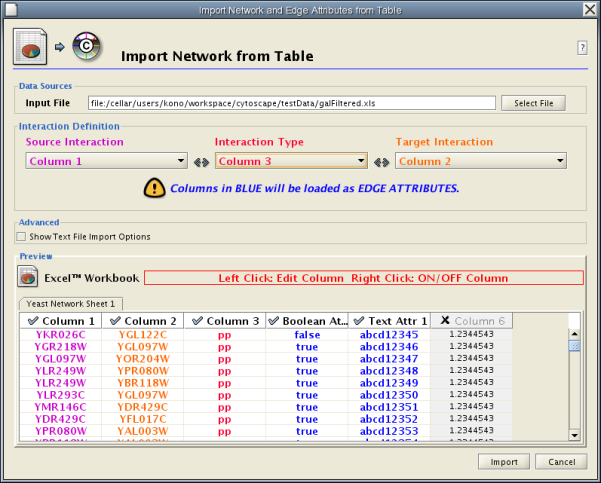
\includegraphics[width=.8\textwidth]{images/network_table_import.png} 
\end{center}

\subsection{支持的文件类型}
``Import Network from Table''功能支持按特定符号分割的文本文件,和单工作表的微软Excel文件。下面就是一个例子:

\medskip

{\center\tiny
\begin{tabular}{cccccc}
source  &target&  interaction&  boolean attribute&  string attribute&        floating point attribute\\
YJR022W &YNR053C &pp     & TRUE  &  abcd12371    &   1.2344543\\
YER116C &YDL013W &pp     & TRUE   & abcd12372    &   1.2344543\\
YNL307C &YAL038W &pp     & FALSE  & abcd12373    &   1.2344543\\
YNL216W &YCR012W &pd     & TRUE   & abcd12374    &   1.2344543\\
YNL216W &YGR254W &pd     & TRUE   & abcd12375    &   1.2344543
\end{tabular}}


网络文件至少要有两列:一列是起点,一列是终点。相互作用的类型是可选的。所以,最简单的网络表格应该是这样的:

\begin{verbatim}
YJR022W YNR053C
YER116C YDL013W
YNL307C YAL038W
YNL216W YCR012W
YNL216W YGR254W
\end{verbatim}

在网络文件中,每一行都是一条边以及这条边的属性。所以,网络文件是网络数据和边属性的组合。当然,表中的某些列可能并不是边的属性。遇到这种情况,就可以选择不导入这些列,在预览窗口中点击这一列的表头就是了。例如,在导入下面这种表时,这个功能有很有用:

\begin{verbatim}

Unique ID A  Unique ID B  Alternative ID A
Alternative ID B  Aliases A Aliases B Interaction
detection methods   First author surnames   Pubmed
IDs   species A species B Interactor types  Source
database Interaction ID  Interaction labels
Cross-references  Associated Files  Experiment
files  Experiment labels Different techniques
Different Pubmed articles Different sources Weight

7205 5747 TRIP6   PTK2 Q15654  Q05397-1  vv|HPRD
Currently not available
14688263|15892868(Marcotte)  Mammalia  Homo
sapiens protein|protein HPRD|Marcotte   0 Thyroid
hormone receptor interactor 6-FAK-|PTK2-TRIP6
NA(HPRD)|NA(Marcotte)
HPRD/02859_psimi.xml|other/ORIGINAL_DATA_MARCOTTE.txt
vv(HPRD/02859_psimi.xml)|HPRD(other/ORIGINAL_DATA_MARCOTTE.txt)
17651(ExptRef)|Marcotte 2 2 2 2

4174 7311 MCM5 UBA52   P33992  P62987
neighbouring_reaction   Currently not available
15608231(Reactome)   Homo sapiens Homo sapiens
protein|protein Reactome  1 P33992-P62988
Reaction:68944<->Reaction:68946(Reactome)|Reaction:68946<->
Reaction:68944(Reactome) other/ORIGINAL_DATA_MARCOTTE.txt
neighbouring_reaction(other/REACTOMEhomo_sapiens.interactions.txt)
Reactome 1 1 1 1

7040 7040 TGFB1   TGFB1   P01137  P01137  nmr:
nuclear magnetic resonance Currently not available
8679613 Homo sapiens Homo sapiens protein|protein
BIND 2 TGFB1-TGFB1- 72085(BIND)
BIND/bind_taxid9606.1.psi.xml   nmr: nuclear
magnetic resonance(BIND/bind_taxid9606.1.psi.xml)
NotAvailable 1 1 1 1

\end{verbatim}

这份数据是用制表符分割的,含有网络数据(相互作用)、边的属性和节点属性。把这份数据导入到~Cytoscape~中,首先选择~Unique ID A~作为起点,Unique ID B~作为目标,Interactor type作为相互作用类型。不要导入节点属性(ALternative ID A、species B等等)。其它的列则作为边的属性导入。

网络导入功能无法导入节点属性,只能导入边属性。关于节点属性的导入,请阅读本手册的~Attributes~一节。


注意:
\begin{enumerate}
	\item 这里的数据来自Andrew Garrow、Yeyejide Adeleye~和~Guy Warner(Unilever, Safety and Environmental Assurance Center, 2006年10月12日)的\emph{A merged human interactome}~数据集。在\url{http://www.cytoscape.orghttp://cytoscape.org/cgi-bin/moin.cgi/Data\_Sets/}上可以下载到真实的数据。
\end{enumerate}

\subsection{基本操作}

导入文本表格或Excel表格中的网络,步骤如下: 
\begin{enumerate}
\item 点击~File $\rightarrow$ Import $\rightarrow$ Network from Table (Text/MS Excel)... 
\item 点击~Select File~按钮,选择一份表格。 
\item 从表格中选择相互作用的起始点和相互作用类型。如果将相互作用的类型设置为缺省类型,则所有的相互作用的类型都会被设为pp;这个参数可以再Advanced Options中修改(下面会介绍)。
\item (可选)如果需要的话,可以定义边属性列。在表格中,除了网络数据,还可以有一些列来表示边的属性。
\begin{itemize}
\item 激活或取消属性列——在预览表格中鼠标左键单击表头,就能激活或去表边的属性。如果表头及该列的内容时蓝色的,则该列将会作为边的属性导入。例如,下面表格中的第1到第3列将会作为网络数据,第4列不会导入,而第5、6两列则会作为边属性导入。
\begin{center}
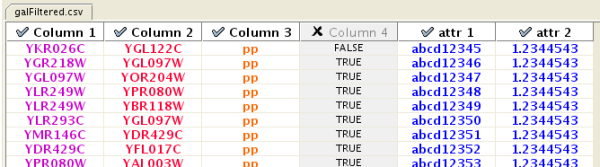
\includegraphics[width=.8\textwidth]{images/network_table_sample.png} 
\end{center}
\item 改变属性名称和数据类型——在预览表格的表头上用鼠标右键单击,就能修改属性的名称和数据类型。有关信息,详见下面的``修改属性名称和类型''。
\end{itemize}
\item 点击~Import按钮。 
\end{enumerate}

\subsection{导入不带边的节点列表}
在~Table Import~中可以导入不带边的节点列表。 如果只选择源节点列,就会创建一个没有相互作用的网络。在使用一些web服务客户端来扩展节点时,这个功能很有用。详细信息,请参阅``从外部数据库中导入网络''。

\subsection{高级选项}
\begin{center}
 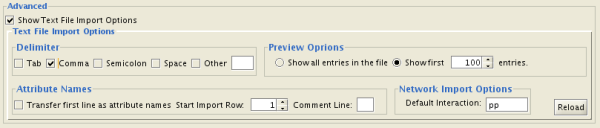
\includegraphics[width=.8\textwidth]{images/network_import_advanced.png} 
\end{center}
选择~Show Text File Import Option~选项,可以对一些选项进行设置。
\begin{itemize}
\item 分隔符(Delimiter):可以为文本表格选择多个分隔符。缺省情况下,分隔符是制表符和空格。
\item 预览选项(Preview Options):选好网络表格文件后,文件中的前一百行数据会显示在预览窗口中。修改这个选项的值,可以在预览窗口中显示更多的内容。如果要显示文件中所有的内容,选上``Show all entries in the file''即可。点击~Reload~按钮可以更新预览窗口中的内容。
\item 属性名称(Attribute Names)
\begin{itemize}
\item 将第一行设为属性名称(Transfer first line as attribute names):选上这个选项,所有的边的属性就会根据表格第一行命名。
\item 起始导入行(Start Import Row):设置从表格中第几行开始导入。例如,如果要忽略文件中的前三行,就可以将这个选项设为4。
\item 注释行(Comment Line:):以该字符开头的行将被视为注释,不会导入。这个选项可以用于跳过文件中的注释。
\end{itemize}
\item 网络导入选项(Network Import Options):如果相互作用的类型被设为缺省相互作用,所有边的类型就会被设为这个值。
\end{itemize}
 
\subsection{修改属性名称和类型}

\begin{center}
 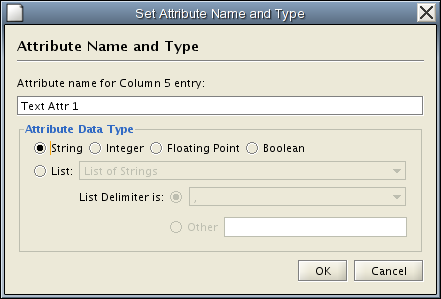
\includegraphics[width=.6\textwidth]{images/network_table_attr_dialog1.png} 
\end{center}

在这里可以修改属性的名称和数据类型。
\begin{itemize}
\item 修改属性名称(Modify Attribute Name):输入新的属性名称,然后点击OK即可。
\item 修改属性数据类型(Modify Attribute Data Type):支持以下数据类型:
\begin{itemize}
\item String 
\item Boolean (True/False) 
\item Integer 
\item Floating Point 
\item List of (one of) String/Boolean/Integer/Floating Point 
\end{itemize}
\end{itemize}
Cytoscape~有基本的数据类型探测功能,能自动地根据该列数据的内容推测数据的类型。不过还是可以自行选择合适的数据类型。对于list,必须要设置一个全局的分隔符(例如,表格中所有的单元格都必须使用相同的分隔符)。

\section{从~Web~服务导入网络}
从~2.6.0~开始,Cytoscape~有了一个新功能\textbf{Web Service~客户端管理器(Web Service Client Manager)}。有了这个功能,用户可以访问各种类型的数据库。
详见\emph{\textbf{从外部数据库导入网络和属性}}。

\section{编辑新网络}
在Cytoscape中还可以新建空网络,然后手动地添加节点和边。点击~File $\rightarrow$ New $\rightarrow$ Network $\rightarrow$ Empty Network,然后可以用CytoPanel 1中的Editor手动的添加网络节点和边(详见Editor一章)。


\chapter{所支持的网络文件格式}
Cytoscape~可以读取以下格式的网络或路径文件:
\begin{itemize}
\item Simple interaction file (SIF or .sif format) 
\item Graph Markup Language (GML or .gml format) 
\item XGMML (extensible graph markup and modelling language). 
\item SBML 
\item BioPAX 
\item PSI-MI Level 1 and 2.5 
\item Delimited text 
\item Excel Workbook (.xls) 
\end{itemize}

SIF~格式的文件只有节点和相互作用,而其它的格式都可以存储网络布局信息,还可以跟其它的网络软件和数据源交换数据。SIF~文件通常用于在新建网络时导入相互作用,因为用文本编辑器和电子表格软件能很方便的创建这种格式的文件。在导入了相互作用,应用了某种网络布局后,就可以将网络存为GML或XGMML格式,从而能去其它系统交换数据。所有的这些格式(Excel例外)都是文本文件,用普通的文本编辑器就能编辑和查看这些文件。


\section{SIF~格式}
这种简单的格式可以很方便地用于从相互作用列表构建网络。利用这种格式,还能很方便的把小网络组合在一起,或是在现有的数据中添加新的相互作用。但这种格式的缺点也是显而易见的,其中不包含布局信息,这使得Cytoscape不得不在每次加载网络时都重新计算网络的布局。

SIF~文件中的每行都由起点、相互作用类型(或边的类型)和一个或若干个重点构成。
\begin{verbatim}
nodeA <relationship type> nodeB
nodeC <relationship type> nodeA
nodeD <relationship type> nodeE nodeF nodeB
nodeG
...
nodeY <relationship type> nodeZ
\end{verbatim}

下面是一个具体的例子:
 \begin{verbatim}
node1 typeA node2
node2 typeB node3 node4 node5
node0
\end{verbatim}

第一行是两个节点,node1和node2,以及两点间的typeA型的相互关系。第二行加入了三个新节点,node3~、\linebreak node4~和~node5,这一行中的node2跟第一行中的node2是同一个节点。第二行还设定了三条起点相同且类型也相同的相互作用。第三行说明了如何引入孤立的节点。 This form is not needed for nodes that do have relationships, since the specification of the relationship implicitly identifies the nodes as well. 

重复的条目被忽略。两个点之间的多条相互作用必须是不同的类型。例如,下面的node1和node2之间就有两条边,但类型分别是xx和yy。
\begin{verbatim}
node1 xx node2
node1 xx node2
node1 yy node2
\end{verbatim}

节点的自相互作用是允许的:
\begin{verbatim}
node1 xx node1
\end{verbatim}

Cytoscape中每个点和每条边都有标识符,通常在节点和边的属性数据中都有。节点的名称必须是独一无二的,名称相同的节点会被视为同一个节点。节点的名称缺省情况下就是文件中的名称,除非用Visual Mapper映射到了其他字符串。详见``视觉风格''一章。边的名称则是由边的起点和终点,加上相互作用的类型构成的,例如:sourceName (edgeType) targetName。


$<$relationship type$>$标签可以是任何字符串。完整的单词或是单词的组合都可以用来定义相互作用的类型,例如:geneFusion、cogInference、pullsDown、activates、degrades、inactivates~、~inhibits~、~phosphorylates~、~upRegulates~等等。 

在系统生物学领域,常见的相互作用类型有:
\begin{enumerate}
\item  pp .................. protein $\rightarrow$ protein interaction
\item  pd .................. protein $\rightarrow$ DNA   
  (例如,转录因子跟调控基因的上游结合。)
\end{enumerate}

还有一些相对少见的相互作用类型:
\begin{enumerate}
\item  pr .................. protein $\rightarrow$ reaction
\item  rc .................. reaction $\rightarrow$ compound
\item  cr .................. compound $\rightarrow$ reaction
\item  gl .................. genetic lethal relationship
\item  pm .................. protein-metabolite interaction
\item  mp .................. metabolite-protein interaction
\end{enumerate}


\textbf{分隔符}

在简单的相互作用文件格式中,空白(空格或制表符)用来分割名称。但在有些情况,节点名称或是边的类型中会含有空格。Cytoscape对分隔符的处理原则是这样的:如果文件中有制表符,那么就用制表符分割不同的字段,而空格则被视为字段中的内容。如果文件中没有制表符,那么所有的空格就都是分隔符(也就是中字段中不会有空格)。

如果在导入网路后,发现网络中没有边,而且点的名称也有问题,那很有可能是因为文件中存在制表符,使得Cytoscape在导入网络时判断错误。另一方面,如果网络中节点的名称只是正确名称的一部分,那就很有可能是错误地将空格作为了分隔符,实际上应该用制表符。

用简单的相互作用的形式存放网络的文件的后缀是.sif,Cytoscape能识别出文件夹中所含有的这类文件。

\section{GML~格式}
跟SIF格式不同,GML是一种富图格式语言(rich graph format language),很多网络可视化软件包都支持这种格式。在\url{http://www.infosun.fmi.uni-passau.de/Graphlet/GML/}上可以找到该格式的具体说明。

通常都不必直接修改GML文件的内容。当SIF格式的网络导入并实施布局后,就可以以GML的形式保存和加载网络。GML文件中的视觉风格在加载GML文件后,会保存为名为Filename.style的视觉风格。

\section{XGMML~格式}
XGMML是GML的XML扩展版,它是基于GML定义的。除了网络数据,XGMML还包含节点、边和网络的属性。XGMML文件的规范在\url{http://www.cs.rpi.edu/~puninj/XGMML/}上。

由于XGMML继承了XML文件的灵活性,所以XGMML比GML更受欢迎。如果不确定应该用哪种格式,那就选择XGMML吧。

\section{系统生物学标记语言(Systems Biology Markup Language)}
系统生物学标记语言(Systems Biology Markup language)是一种用于描述生化网络的XML格式。SBML文件格式规范:\url{http://sbml.org/documents/}
 
\section{BioPAX (Biological PAthways eXchange)格式}

BioPAX是一种用于交换生物路径数据的OWL(Web Ontology Language)文档。该格式的完整说明文档:\url{http://www.biopax.org/index.html}

\section{PSI-MI~格式}
PSI-MI格式一种用于描述蛋白质相互作用及有关数据的XML格式。PSI-MI XML的格式规范:
\url{http://psidev.sourceforge.net/mi/xml/doc/user/}。

\section{纯文本表格和Excel表格}

Cytoscape~为微软的Excel文件(.xls)和纯文本表格提供了原生支持。可以用这些表格存储网络数据和边的属性。在导入文件的过程中,用户可以指定哪一列是源节点,哪一列是终点,以及相互作用的类型、边属性等等。其它的一些网络分析工具,例如igraph (\url{http://cneurocvs.rmki.kfki.hu/igraph/}), 也可以将网络输出成简单的文本文件。Cytoscape~可以读取这些文本文件,并构建网络。具体信息请阅读\ref{free-format table} 节。

\centerline{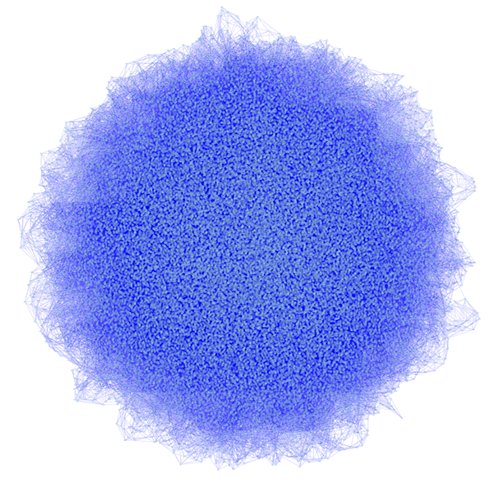
\includegraphics[width=.7\textwidth]{images/huge_network_igraph.png}}

\textbf{在Cytoscape中显示根据~igraph~的Watts-Strogatz小世界模型生成的网络(含有5万个节点,25万条边)}
 
利用Table Import功能,可以读取其它软件生成的网络。
 
\section{Cytoscape~中节点的命名}

通常情况下,节点表示基因,节点间的边表示相互作用(或者是其他的生物关系)。
为了紧凑,基因也可以表示成响应的蛋白质。节点还可以用来表示化合物和生化反应等各种
东西,并不局限于基因。

如果想要将网络中的基因或蛋白跟GO注释或基因表达数据整合在一起,那各个数据文件中的基因名称
必须完全一致。我们强烈建议用户用ORF系统名称或是标准的获取编号(accession number)来命名
基因和蛋白质。而常用名称(common name)由于更适合显示在屏幕上,所以可以将其存放在注释目录或
节点的属性文件中。Cytoscape的annotation/目录中中有酵母的ORF到常用名称的对应文件。将来会逐步
地支持其它物种。

为什么要建议使用标准的基因名称?所有~Cytoscape~能识别的外部数据格式都有专门的命名方式。例如,
蛋白质相互作用网络会列出蛋白质的名称,相应的属性和表达数据也使用同样的命名方法。

但如果要把不用来源的数据结合在一起,问题就出现了:对于同一个东西,不同的数据源的命名可能
是不一样的。例如,基因就可以有多个不同的名称,包括正式的``染色体位置''标识符,研究人员讨论
时常用的若干个名称。此外,每个数据库可能还会有自己的一套给基因编号的方法(例如Swiss-Prot的
蛋白质编号)。如果一个数据源使用的是正式名称,而另一个数据使用的是常用名称,那Cytoscape就必须
要知道哪两个名称指的是同一个基因。

有两种方法来解决这个问题,一个较简单,另一个稍微复杂一些。简单的方法就是假设所有的数据源使用同样
的命名方法。如果是这样,Cytoscape就能很方便的将来自不同数据源的数据结合在一起。

跟人工整合不同来源的数据一样,为了处理不同命名方式的数据,Cytoscape需要同义词信息(见``注释
''一章)。同义词表提供了某个物种的每个对象的权威名称,以及相应的其它可以识别的名称。要注意,同义词表
自身的数据就是按照这个``权威''名称命名的。例如,在酵母中,通常用ORF名称作为这个``权威''名称。

如果能提供这样信息,Cytoscape在缺省情况下会将所有的名称都转换成相应的权威名称。而不能识别的名称
则保持不变。这样Cytoscape就能将不同来源的数据结合在一起,即使它们的名称不同也没关系---只要能在同义词
表中找到就行。

For this to work, Cytoscape must also be provided with the species to which
the objects belong, since the data server requires the species in order to
uniquely identify the object referred to by a particular name. This is usually
done in Cytoscape by specifying the species name on the command line with the
-P option (cytoscape.sh -P ``defaultSpeciesName=Saccharomyces
cerevisiae'') or by editing the properties (under Edit $\rightarrow$ Preferences
$\rightarrow$ Properties\ldots). 

The automatic canonicalization of names can be turned off using the -P option
(cytoscape.sh -P ``canonicalizeName=false'') or by editing the properties (under
Edit $\rightarrow$ Preferences $\rightarrow$ Properties\ldots). This canonicalization
of names currently does not apply to expression data. Expression data should
use the same names as the other data sources or use the canonical names as
defined by the synonym table. 


\chapter{节点和边的属性}
相互作用网络是很有用的模型,但是,如果能跟其它信息整合在一起,则能解答更多的科学疑问。在Cytoscape中,用户可以给节点、边或网络添加各种属性。例如,可以是基因的注释数据或蛋白质相互作用的可信度。这些属性可以按着用户的设置映射到可视化属性上(颜色、形状等等)。本节会详细介绍视觉风格。

\section{Cytoscape~属性文件格式}
节点和边的属性文件的格式非常简单:节点属性文件的第一行是属性的名称(注意,属性名称中不能有空格)。接下来的每一行首先是节点的名称,然后是等号,以及属性的值。最常见的属性类型是数字和字符串。同一个属性的所有值都必须是同一类型的。例如:

 \begin{verbatim}
FunctionalCategory
YAL001C = metabolism
YAR002W = apoptosis
YBL007C = ribosome
\end{verbatim}

边的属性文件也类似,不同的是边的名称是由起点名称,加上括号中的边的类型,然后是重点名称构成的。边是有方向性的,所以交换起点和终点的位置会被认为是不同的边(有可能是不存在的)。下面就是一个边属性文件的例子:

 \begin{verbatim}
InteractionStrength
YAL001C (pp) YBR043W = 0.82
YMR022W (pd) YDL112C = 0.441
YDL112C (pd) YMR022W = 0.9013
\end{verbatim}

在Cytoscape中,边是有方向的,所以上表中的第三行和第四行表示的是两条不同的边(涉及到的节点是一样的,但终点和起点是相反的)。

每个文件存放一个属性。节点和边的属性文件的格式是一样的。节点属性文件名的后缀一般是
``.noa'',边属性文件名的后缀通常是``.eda''。这两个后缀都能被Cytoscape识别。

可以用命令行的-n和-e选项或菜单中的File $\rightarrow$ Import加载节点和边的属性。

如果通过基因表达矩阵加载了基因表达数据,在缺省情况下,其表达值会自动地转换成节点的属性。

节点和边的属性只跟节点和边有关,是独立于网络的。无论是先加载网络文件还是先加载属性文件,节点或边的属性都会应用到当前加载的所有网络中。

\textbf{注意:}在Cytoscape 2.4中导入网络属性时,请使用File $\rightarrow$ Import $\rightarrow$ Attribute from Table (text/MS Excel)...或XGMML格式的网络文件(相见所支持的文件格式一章)。

\subsection{符号分割文件格式(高级用户)}

该格式的属性文件的第一行说明了属性的名称以及该属性的附加信息,如下:

\begin{verbatim}
attributeName (class=formal.class.of.value)
\end{verbatim}

第一个字段必须是属性名称,并且不能含有空格。class字段定义了属性值的正式类型。例如,
java.lang.String表示字符串、java.lang.Double表示浮点数值、java.lang.Integer表示整数,以此类推。
如果值是一份列表,那么class字段就应该是列表中对象的类型。如果没有指定class字段,Cytoscape
就会根据文件中的第一个值猜测其类型。如果第一个值中含有浮点格式的数字,Cytoscpae就会认为是
java.lang.Double;如果第一个值只有数字,没有小数点,Cytoscape就会认为是java.lang.Integer;除此以外,Cytoscape
都会将其视为java.lang.String。所以,要小心,第一个值可能会造成Cytoscape的错误,例如:

 \begin{verbatim}
floatingPointAttribute
firstName = 1
secondName = 2.5
\end{verbatim}

在上面的例子中,第一个值会导致Cytoscape将该属性的类型设为整数,但实际上其类型应该是
浮点数。所以最好是明确地指定属性的类型,以避免这种错误。如下:

 \begin{verbatim}
floatingPointAttribute (class=Double)
firstName = 1
secondName = 2.5
\end{verbatim}

或者:

 \begin{verbatim}
floatingPointAttribute 
firstName = 1.0
secondName = 2.5
\end{verbatim}

在第一行之后,每一行首先是对象的名称(在节点属性文件中就是节点名称,在边属性
文件中就是边的名称),然后是该属性的值。分隔符是等号,等号前后的空格(包括中
制表符)都会被忽略。在名称和值中可以有空格,但名称中不能含有等号,开头结尾也
不能有空白。对象名称必须跟属性浏览器中的节点名称或边名称完全一致,包括大小写,
否则就会匹配不上。

边的名称的形式如下:

\begin{verbatim}
sourceName (edgeType) targetName
\end{verbatim}

具体来说,就是: 

\begin{verbatim}
起点名称 空格 括号 边类型 括号 空格 终点名称
\end{verbatim}

注意,在边的名称中不能含有制表符。可以用制表符将边名称和``=''分隔符隔开,但边的名称里面不能含有
制表符。此外,还要注意,这里的格式跟SIF文件的格式是不一样的。SIF文件中的相互作用的格式如下:

 \begin{verbatim}
sourceName edgeType targetName
\end{verbatim}

即:

\begin{verbatim}
起点名称 空格 边类型 空格 终点名称
\end{verbatim}

设置一系列值的语法如下:

 \begin{verbatim}
listAttributeName (class=java.lang.String)
firstObjectName = (firstValue::secondValue::thirdValue)
secondObjectName = (onlyOneValue)
\end{verbatim}

这个例子展示的属性的值是一系列的字符串。第一个对象有三个字符串,所以列表中有三个元素,而第二个对象的列表则只有
一个元素。在属性为列表的情况下,所有的属性值都应该使用列表语法(例如,括号),
每个元素的类型也必须一样。再提醒一下,如果没有在第一行中说明属性值的类型的话,
Cytoscape会尝试猜测其类型。列表类型的属性不能映射到视觉属性上。

\subsection{断行功能}
在某些情况下,属性中会含有断行,例如节点的标签太长。在属性值中插入``\\n''就能
实现断行。例如:

\begin{verbatim}
newlineAttr
YJL157C = This is a long\nline for a label.
\end{verbatim}

\section{导入属性表格文件}
从Cytoscape 2.4开始,就可以导入符号分割文件和微软的Excel表格数据。有了这个功能,用户可以
方便地将原来不被Cytoscape支持的节点或边属性文件导入到Cytoscape中。

\centerline{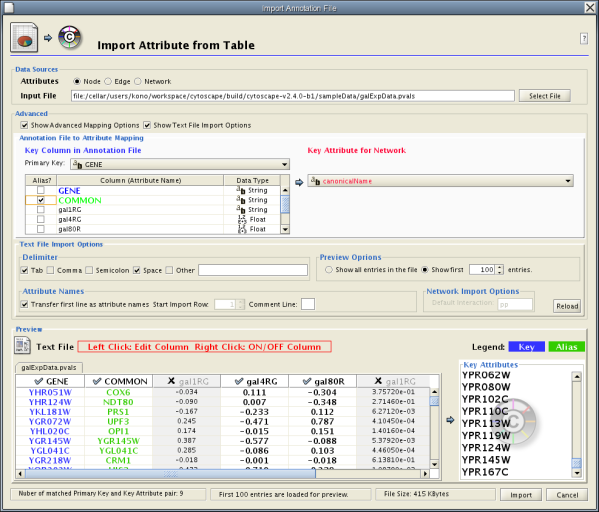
\includegraphics[width=.4\textwidth]{images/attribute_table_import_main.png} }

\begin{tabular}{|c|c|c|}
\hline 
 Object& Key Alias& SGD ID\\
\hline
 AAC3 &YBR085W|ANC3& S000000289\\
 AAT2 &YLR027C|ASP5& S000004017\\
 BIK1 &YCL029C|ARM5|PAC14 &S000000534\\
 \hline 
\end{tabular}

属性表文件应该含有主键列,最少有一列属性。属性列的数量没有限制。因为默认会将数据的第一行作为属性名称,所以Alias(别名)列是可选的。当然也可以在
File$\rightarrow$Import$\rightarrow$Attribute from Table (text/MS Excel)...
的用户界面中指定每一列属性的名称。

\subsection{基本操作}
``Import Attributes from Table''窗口的用户界面跟
``Import Network from Table''窗口的界面类似. 
\begin{enumerate}
\item 选择File $\rightarrow$Import $\rightarrow$Attribute from Table (text/MS
Excel)... 
\item 从Attributes单选按钮中选择一种属性类型,Cytoscape可以导入节点、边和网络属性。
\item 选择数据文件。 点击Select File按钮,加载本地的纯文本文件或Excel(.xls)文件。在文本框中输入远程文件的URL就能加载远程文件。点击Show Text File Import Options面板中的Reload按钮能显示远程文件的预览。
\item (可选) 如果表格分割不正确,可以调整
Text File Import Options面板中的分隔符。缺省的分隔符是制表符。
对于Excel文件则不需要这一步。
\item 缺省情况下,第一列属性是主键。有必要的话可以修改。\\
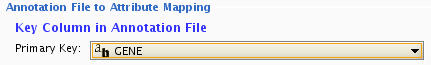
\includegraphics[width=0.3\textwidth]{images/attribute_table_import_primary_key.png} 
\item 点击Import按钮。 
\end{enumerate}
 
\subsection{高级选项}
\subsubsection{Mapping Key Attributes to the primary key}
Formerly, Cytoscape only supported mapping between node/edge IDs and the
primary keys in attribute files. With the introduction of Cytoscape 2.4, this
limitation has been removed, and now both IDs and attributes with primitive
data types (string, boolean, floating point, and integer) can be selected as
the Key Attribute using the dropdown list provided. Complex attributes such as
lists are not supported. 

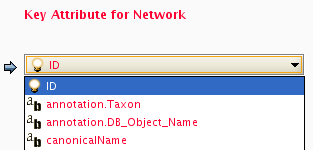
\includegraphics[width=.3\textwidth]{images/attribute_table_import_keyattr.png} 
 
\subsubsection{别名}
Cytoscape uses a simple mechanism to manage aliases of objects. Both nodes and
edges can have aliases. If an attribute is loaded as an alias, it is treated as
a special attribute called ``alias''. This will be used when mapping
attributes. If the primary key and key attribute for an object do not match,
Cytoscape will search for a match between aliases and the key attribute. To
define an alias column in the attribute table, just click on the checkboxes to
the left of the column name while importing. 

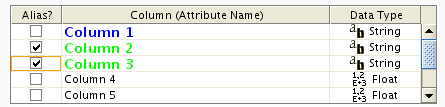
\includegraphics[width=.3\textwidth]{images/attribute_table_import_alias.png} 
 
\subsubsection{文本文件导入选项}
For more detail on these options, please see the ``Import Free-Format Table
Files'' section of the user manual in the Creating Networks chapter. 

\subsection{属性浏览器}
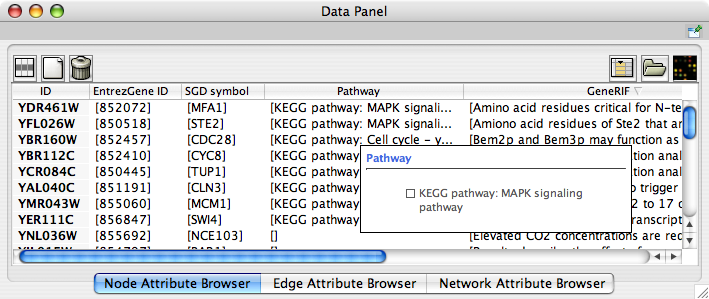
\includegraphics[width=.5\textwidth]{images/attribute_browser26.png} 
 
When Cytoscape is started, the Attribute Browser appears in the bottom
CytoPanel. This browser can be hidden and restored using the F5 key or the View
$\rightarrow$ Show/Hide attribute browser menu option. Like other CytoPanels, the
browser can be undocked by pressing the little icon in the browser's
top right corner. 

 To swap between displaying node, edge, and network attributes use the tabs on
the bottom of the panel labelled ``Node Attribute Browser'', ``Edge Attribute
Browser'', and ``Network Attribute Browser''. The attribute browser displays
attributes belonging to selected nodes and/or edges and the currently selected
network. To populate the browser with rows (as pictured above), simply select
nodes and/or edges in a loaded network. By default, only the ID of nodes and
edges is shown. To display more than just the ID, click the Select Attributes

\includegraphics[width=1em]{images/attributes_select_icon.png}  button and choose
the attributes that are to be displayed (select various attributes by clicking
on them, and then click elsewhere on the screen to close the attribute list).
Each attribute chosen will result in one column in the attribute browser. Most
attribute values can be edited by double-clicking an attribute cell; list
values cannot be edited, and neither can the ID. Attribute rows in the browser
can be sorted alphabetically by specific attribute by clicking on a column
heading. A new attribute can be created using the Create New Attribute

\includegraphics[width=1em]{images/attributes_new_icon.png}  button, and must be
one of four types \^a€“ integer, string, real number (floating point), or
boolean. Attributes can be deleted using the Delete Attributes
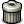
\includegraphics[width=1em]{images/attributes_delete_icon.png}  button.
\textbf{NOTE: Deleting attributes removes them from Cytoscape, not just the
attribute browser!} To remove attributes from the browser without deleting
them, simply unselect the attribute using the Select Attributes

\includegraphics[width=1em]{images/attributes_select_icon.png}  button. 

The right-click menu on the Attribute Browser has several functions, such as
exporting attribute information to spreadsheet applications. For example, use
the right-click menu to Select All and then Copy the data, and then paste it
into a spreadsheet application. Each attribute browser panel also has a button
for importing new attributes:

\includegraphics[width=1em]{images/attributes_import_icon.png}  . 

 The Node Attribute Browser panel has additional buttons for loading Gene
Expression attribute matrices (
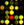
\includegraphics[width=1em]{images/attributes_gene_expr_icon.png}  ) as node
attributes. 

\subsubsection{属性批量编辑器}
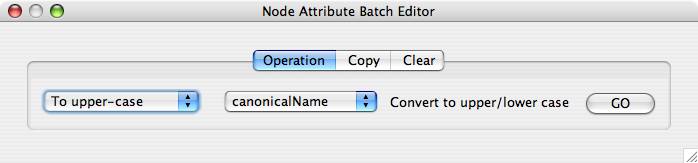
\includegraphics[width=.5\textwidth]{images/attribute_editor26.png} 

From Cytoscape 2.6, Attribute Browser has new \textbf{Attribute Batch Editor}
. This enables you to set and modify attribute values at once. This function
changes values for selected nodes or edges. For example, if you want to create
a new attribute called \emph{Modules} and set module names for each group of
selected nodes, you can use \emph{Set} command from this editor. 


\chapter{加载基因表达(属性矩阵)数据}
除了普通的节点和边属性数据,Cytoscape~还支持导入基因表达数据。基因表达数据的格式跟一般的属性文件的格式不一样,但是对于Cytoscape来说,最终对这些属性的处理方法却没有区别。基因表达数据(跟属性数据一样)在任何时候都可以导入,但(通常)都是在网络加载后导入一次。 

\section{数据文件格式}
一个或多个实验所得到的基因表达比例(gene expression ratio)或称基因表达值(value)都是用文本文件存储的。比例结果来自于两个基因表达测试(实验组和对照组)的比较。在某些基因表达平台上,例如Affymetrix,可以直接测出基因表达值,而无需比较。文件包括一个头部,以及若干用空格或制表符分割的域,每一行都是一个基因,大概的格式如下:
\begin{verbatim}
Identifier [CommonName] value1 value2 ... valueN [pval1 pval2 ... pvalN]
\end{verbatim}
方括号\[ \]表示该域是可选的。

第一个域用于识别该基因对应Cytoscape中的哪个节点。在最简单的情况下,这就是基因的名称,跟其在Cytoscape中的网络中的名称完全一致(大小写敏感)。此外,也可以是能识别节点的某些属性,例如商业微阵列的探针标识。

接下来的一个域是常见名称,可选的。这对于Cytoscape并没有什么用,只是用户的习惯而已。有了这个CommonName域,该输入文件的格式就跟其它的常见的基因表达数据分析包一致了,例如SAM(\url{http://www-stat.stanford.edu/~tibs/SAM/})。 

接下来的就是各个实验所测得的基因表达值。这些值可以使绝对的基因表达值,也可以fold change的比例。可以根据第一行中的实验名称来区分各个实验。

还有一个可选的值表示显著程度的P值。很多阵列数据分析包都能计算出这个值,表示基因表达或fold change较随机情况的显著程度。显著度会列在基因表达数据后面。显著度的名称应该跟基因表达数据的实验名称完全一致。

看一个例子,下面是Cytoscape的sampleData目录中galExpData.pvals文件的节选:
\begin{verbatim}
GENE COMMON gal1RG gal4RG gal80R gal1RG gal4RG gal80R
YHR051W COX6 -0.034 0.111 -0.304 3.75720e-01 1.56240e-02 7.91340e-06
YHR124W NDT80 -0.090 0.007 -0.348 2.71460e-01 9.64330e-01 3.44760e-01
YKL181W PRS1 -0.167 -0.233 0.112 6.27120e-03 7.89400e-04 1.44060e-01
YGR072W UPF3 0.245 -0.471 0.787 4.10450e-04 7.51780e-04 1.37130e-05
\end{verbatim}
在这个数据中有三个实验:gal1RG,gal4RG和gal80R。这三个名称在表头中出现了两次,首先是基因表达值,然后是显著度。例如,从第二行数据可知,在gal1RG试验中,YHR051W的基因表达值是-0.034,显著度是3.75720e-01。

在基本格式上还能有一些变动,详见下面的文件格式说明。基因表达数据文件通常的后缀是``.mrna''或``.pvals'',这些文件都能被Cytoscape识别。
\section{基本过程}
用File $\rightarrow$ Import $\rightarrow$ Attribute/Expression Matrix...加载基因表达矩阵数据,会弹出导入窗口;还可以用命令行选项-m指定基因表达数据文件。如果用命令行加载基因表达数据,则基因表达数据必须按照节点ID输入。如果用对话框,可以根据节点的ID加载基因表达数据(缺省),也可以根据其他的节点属性加载基因表达数据。如果使用某个节点属性,该属性必须满足(1)该属性已经加载了;(2)该属性必须跟基因表达举证文件第一行相匹配。
 
\section{实例}
下面针对sampleData/galFiltered.sif网络演示一下如何导入基因表达数据: 
\begin{enumerate}
\renewcommand{\labelenumi}{\textbf{Option \Alph{enumi}.}}
\item 点击File $rightarrow$ Import $rightarrow$ Attribute/Expression Matrix\ldots 。在结果窗口中,有一个名为``Please select an attribute or expression matrix file\ldots'',用Select按钮输入sampleData/galExpData.pvals。这个文件中的标识符和sampleData/galFiltered.sif网络数据中的标识符是一致的,所以不需要使用``Assign values to nodes using...''。下面是这个文件中的几行内容:
\begin{verbatim}
GENE COMMON gal1RG gal4RG gal80R gal1RG gal4RG gal80R
YHR051W COX6 -0.034 0.111 -0.304 3.75720e-01 1.56240e-02 7.91340e-06
YHR124W NDT80 -0.090 0.007 -0.348 2.71460e-01 9.64330e-01 3.44760e-01
YKL181W PRS1 -0.167 -0.233 0.112 6.27120e-03 7.89400e-04 1.44060e-01
\end{verbatim}
\item 第1步:在加载网络后,再用File$\rightarrow$Import$\rightarrow$Node attributes\ldots加载sampleData/gal.probeset.na中的节点属性。下面是这个文件的部分内容:
\begin{verbatim}
Probeset
YHR051W = probeset2
YHR124W = probeset3
YKL181W = probeset4
\end{verbatim}
第2步:在加载了节点属性文件后,选择基因表达数据文件sampleData.galExpPvals.probeset.pvals,下面是该文件的部分内容: 
 \begin{verbatim}
GENE COMMON gal1RG gal4RG gal80R gal1RG gal4RG gal80R
probeset2 COX6 -0.034 0.111 -0.304 3.75720e-01 1.56240e-02 7.91340e-06
probeset3 NDT80 -0.090 0.007 -0.348 2.71460e-01 9.64330e-01 3.44760e-01
probeset4 PRS1 -0.167 -0.233 0.112 6.27120e-03 7.89400e-04 1.44060e-01
\end{verbatim}
在选择了文件后,在``Assign values to nodes using...''中选择~Probeset。这会导入跟前一个例子中完全一样的基因表达数据,但在节点名称不能用作标识符的情况下,这会更加灵活。
\end{enumerate}
\section{文件格式的详细说明(高级用户)}
在基因表达数据文件中,任何空白(空格或制表符)都被视为相邻域的分隔符。数据中的各行只有可能是表头或是某个基因的各个测量值。名称转换不适用于基因表达数据文件。

基因表达数据中第一列给出的名称必须跟其它地方所使用的基因名称完全一致(例如SIF或GML文件)。

第一行是表头行,格式有以下三种:
\begin{verbatim}
<text> <text> cond1 cond2 ... cond1 cond2 ... [NumSigConds]
<text> <text> cond1 cond2 ...
<tab><tab>RATIOS<tab><tab>...LAMBDAS
\end{verbatim}
第一种格式中既有基因表达比例,也有显著度。前两个尖括号中的是基因的名称,例如正式名称和常见名称。
The first format specifies that both expression ratios and significance values
are included in the file. The first two text tokens (in angled brackets)
contain names for each gene, such as the formal and common gene names. The
condX token set specifies the names of the experimental conditions; these
columns will contain ratio values. This list of condition names must then be
duplicated exactly, each spelled the same way and in the same order.
Optionally, a final column with the title NumSigConds may be present. If
present, this column will contain integer values indicating the number of
conditions in which each gene had a statistically significant change according
to some threshold. 

The second format is similar to the first except that the duplicate column
names are omitted, and there is no NumSigConds field. This format specifies
data with ratios but no significance values. 

The third format specifies an MTX header, which is a commonly used format. Two
tab characters precede the RATIOS token. This token is followed by a number of
tabs equal to the number of conditions, followed by the LAMBDAS token. This
format specifies both ratios and significance values. 

Each line after the first is a data line with the following format: 
\begin{verbatim}
FormalGeneName CommonGeneName ratio1 ratio2 ... [lambda1 lambda2 ...] [numSigConds]
\end{verbatim}

The first two tokens are gene names. The names in the first column are the keys
used for node name lookup; these names should be the same as the names used
elsewhere in Cytoscape (i.e. in the SIF, GML, or XGMML files). Traditionally in
the gene expression microarray community, who defined these file formats, the
first token is expected to be the formal name of the gene (in systems where
there is a formal naming scheme for genes), while the second is expected to be
a synonym for the gene commonly used by biologists, although Cytoscape does not
make use of the common name column. The next columns contain floating point
values for the ratios, followed by columns with the significance values if
specified by the header line. The final column, if specified by the header
line, should contain an integer giving the number of significant conditions for
that gene. Missing values are not allowed and will confuse the parser. For
example, using two consecutive tabs to indicate a missing value will not work;
the parser will regard both tabs as a single delimiter and be unable to parse
the line correctly. 

Optionally, the last line of the file may be a special footer line with the
following format: 
 \begin{verbatim}
NumSigGenes int1 int2 ...
\end{verbatim}
This line specified the number of genes that were significantly differentially
expressed in each condition. The first text token must be spelled exactly as
shown; the rest of the line should contain one integer value for each
experimental condition. 


\chapter{从外部数据库导入网络和属性}
\section{Web服务客户端管理器}
Cytoscape 2.6的一项新功能就是Web服务客户端管理器(Web Service Client Manager)。这是一个用于管理Cytoscape中各种Web服务的框架。通过Web服务客户端,用户可以方便地访问各种远程数据资源。

\subsection{什么是Web服务?}
Web服务是网络上一种标准化的,平台无关的交互机制。现在主流的生物数据库都通过Web服务API发布数据。
\begin{itemize}
\item 生物Web服务清单:http://taverna.sourceforge.net/services
\item EBI的Web服务:http://www.ebi.ac.uk/Tools/webservices/
\end{itemize}

开发人员可以编写程序访问这些服务。Cytoscape用这个框架开发了一些简单的Web服务客户端。Cytoscape支持的Web服务包括:
\begin{itemize}
\item PSICQUIC:生物相互作用数据的标准Web服务。截止2010年七月,PSICQUIC支持以下数据:
\begin{itemize}
\item  APID
\item    ChEMBL
\item    BioGrid
\item    InnateDB
\item    DIP
\item    IntAct
\item    MatrixDB
\item    MPIDB
\item    Reactome
\item    Reactome-FIs
\item    MINT
\item    iRefIndex
\item    STRING 
\end{itemize}
\item Pathway Commons:访问多种集成数据集的门户,包括Reactome, IntAct, HPRD, HumanCyc, MINT, the MSKCC Cancer Cell Map, 和NCI/Nature Pathway Interaction数据库。
\item NCBI Entrez Gene:关于基因的公共数据,包括注释、序列和相互作用。
\item Biomart:开源生物数据库引擎。可用于ID和名称的映射。
\end{itemize}

所有的这些客户端都有相应的插件,用户可以在插件管理器(Plugin Manager)中安装。

在下面几节中,我们会学习如何从外部数据库导入网络。

\section{快速入门}
首先,选择File$\rightarrow$Import$\rightarrow$Networks from web services\ldots

\centerline{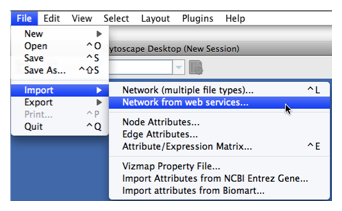
\includegraphics[width=.5\textwidth]{images/file_import.png}}

\centerline{\framebox{提示:从Web服务导入网络,见\href{http://cbio.mskcc.org/~cerami/cytoscape/CytoWebServices.mov}{动画演示}。}}

\section{例子1:从IntAct获取蛋白质相互作用网络}
\begin{itemize}
\item 选择:File$\rightarrow$Import$\rightarrow$Network from web services\ldots
\item 从下拉菜单中选择IntAct Web Service Client。
\item 输入一个或多个搜索词,例如BRCA1。
\item 点击Search按键。
\end{itemize}

\centerline{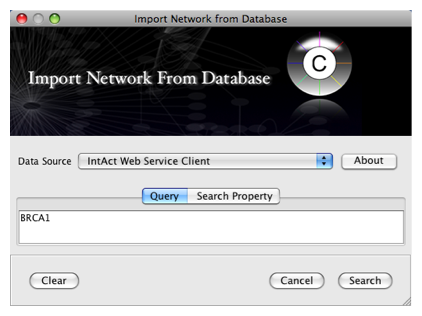
\includegraphics[width=.5\textwidth]{images/intact_import.png}}

在完成相互作用数据的下载后,BRCA1的网络就会导入Cytoscape并显示。

\centerline{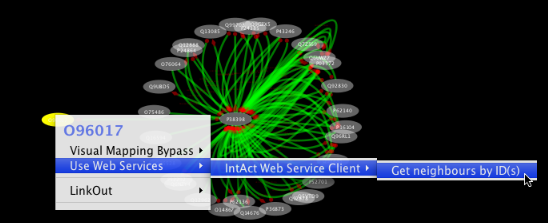
\includegraphics[width=.5\textwidth]{images/node_context2.png}}

{\bf 提示:扩展网络:}很多Cytoscape Web服务都在节点的弹出菜单中提供了一些选项。在节点上点击鼠标右键,选择``Use Web Service''。例如,在上面的截图中,我们从IntAct加载了BRCA1的网络,然后选择将节点的邻居节点添加到网络中。


\section{例子2:从NCBI Entrez Gene获取蛋白质相互作用网络}
在NCBI Entrez Gene记录中,有一段信息叫做interaction。NCBI Web服务客户端就是利用这段信息来构建网络。
\begin{itemize}
\item 选择:File$\rightarrow$Import$\rightarrow$Network from web services\ldots
\item 从下拉菜单中选择NCBI Web Service Client。
\item 输入关键字。例如,human muscular dystrophy(人类肌肉萎缩)
\item 点击Search按钮。
\end{itemize}

\centerline{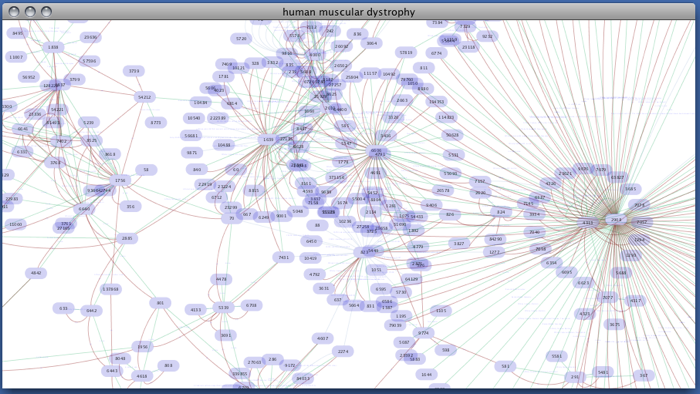
\includegraphics[width=.7\textwidth]{images/entrez_import.png}}

从Entrez Gene数据生成的网络:上图中的网络是从匹配human muscular dystrophy的interaction数据中生成的。边的颜色表示数据的来源(BIND、BioGRID或HPRD)。

{\bf 注意:}因为NCBI客户端需要从海量的数据中抽取相互作用数据,所以它需要较长的时间(30秒到5分钟,取决于机器性能和网速)来导入大量的相互作用数据。


\section{例子3:从Pathway Commons获取通路和网络}


\section{未来发展方向}

\section{从外部数据库导入属性}
\subsection{例子1:从BioMart导入ID和注释}
\subsection{例子2:从NCBI Entrez Gene数据库导入注释}

\section{在工作流中使用多个服务}
\subsection{例子:导入和注释网络}



\chapter{浏览和布局}

\chapter{可视化风格}

\chapter{节点和边的查找与过滤}

\chapter{编辑网络}

\chapter{插件和插件管理器}

\chapter{CytoPanel}

\chapter{渲染引擎}

\chapter{注释}

\chapter{链接}

\chapter*{感谢}

\chapter*{附录A:老式的注释服务器格式}

\chapter*{附录B:GNU Lesser General Public License}

\chapter*{附录C:增加Cytoscape的内存}

\end{CJK}
\end{document}

